\begin{figure}
\centering
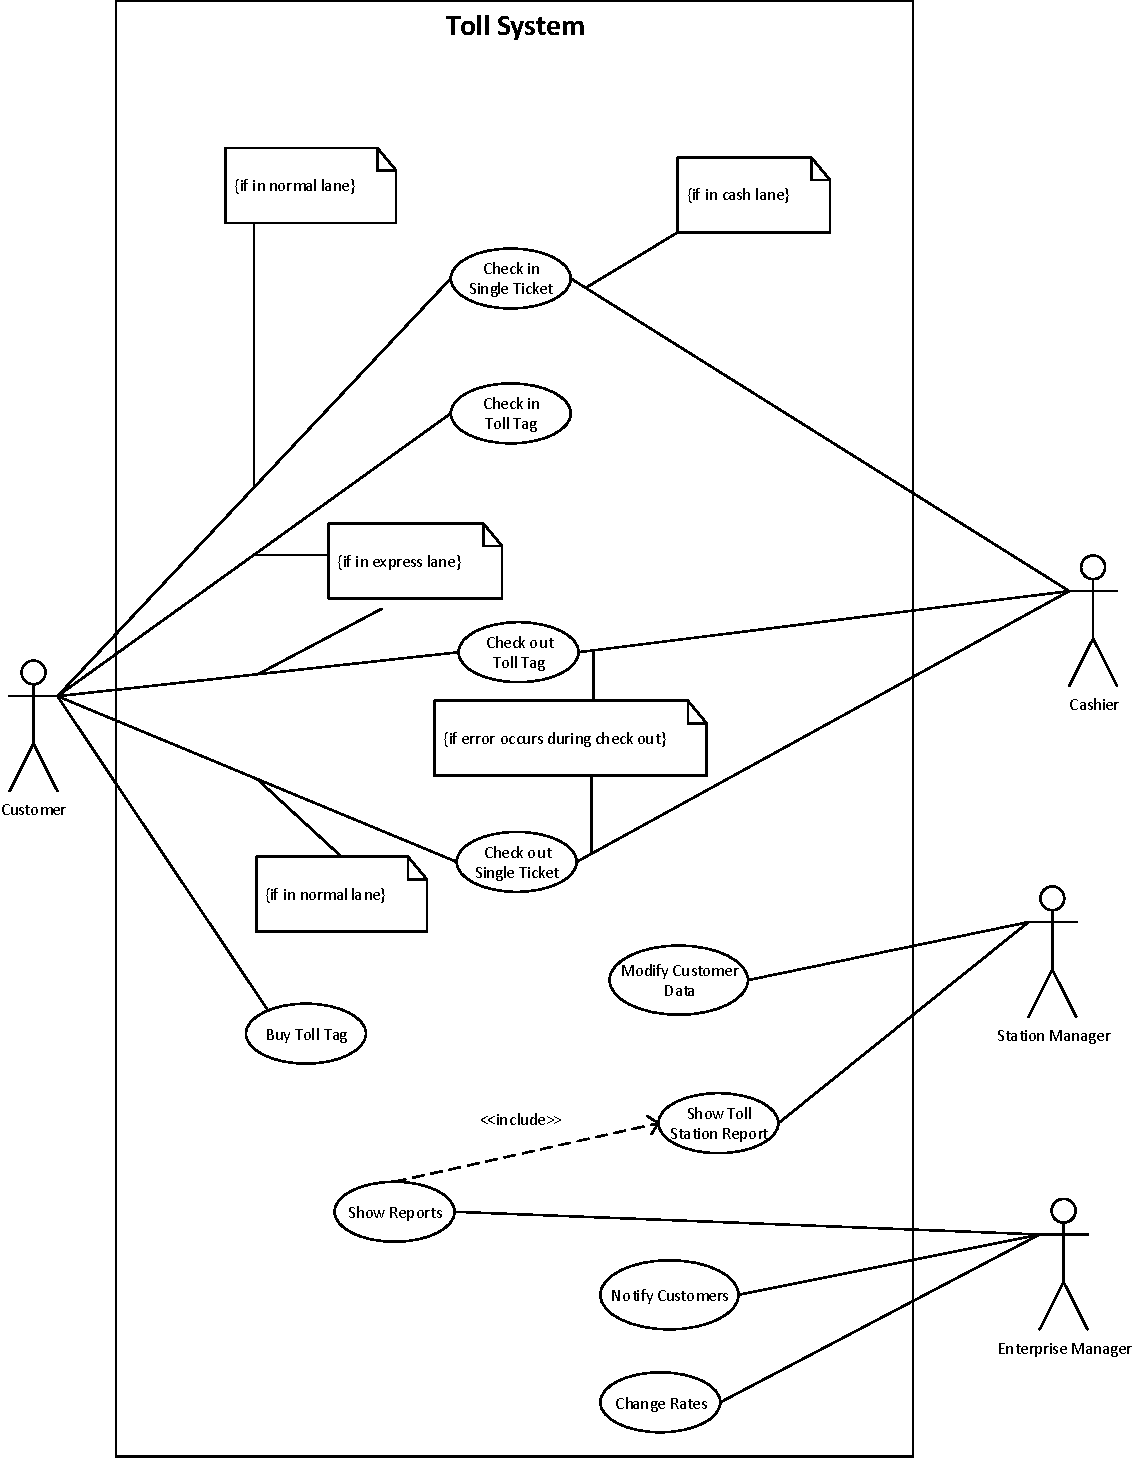
\includegraphics[width=1\textwidth]{img/use_case_diagram/use_case_diagram}
\caption{The use case diagram for the toll system.}
\label{fig:use_case_diagram}
\end{figure}

The use case diagram can be seen in \autoref{fig:use_case_diagram}. It consists of the use cases describing the full functionality of the toll lane system.

We have selected the following use cases, as we have decided that they contain the most important functionality for the owner of the system:
\begin{enumerate}
\item Check in Single Ticket
\item Check out Single Ticket
\item Check in Toll Tag
\item Check out Toll Tag
\item Buy Toll Tag
\item Show Reports
\end{enumerate}

With these use cases both the single tickets and toll tags can be fully used and statistics about the system can be generated by the enterprise manager.
